\documentclass[a4paper,12pt]{report}
%\documentclass[aps,twocolumn,secnumarabic,balancelastpage,amsmath,amssymb,nofootinbib,floatfix]{revtex4-1}
\usepackage[utf8]{inputenc}
\usepackage[a4paper,margin=0.75in]{geometry}
\usepackage{graphicx}
\usepackage{mathrsfs}
\usepackage{amsmath}
\usepackage{amsfonts}
\usepackage{sidecap}
\usepackage{url}

\usepackage{setspace}
\usepackage{wrapfig}

\renewcommand{\thesection}{\arabic{section}}

\begin{document}

\title{Project 4: Analysis of Particle Jets Using Persistent Homology}
\author{Noah Green \\ PHY 480 \\ Michigan State University}
\date{ \today}
\maketitle
\begin{abstract}
 Groups of highly relativistic particle jets can form in particle accelerators when a massive particle decays hadronically. If the massive particle is already moving in a highly boosted reference frame, then the jets from its decay leave the event side-by-side. As particle accelerators evolve to operate at higher energies and make more massive particles, it will be necessary to develop new techniques to tell if a jet is actually composed of a group of these smaller jets. Persistent homology is a relatively new technique that can be used to determine the structure of point clouds, and has the potential to improve current jet analysis techniques on this front. It has the ability to distinguish the distance scales on which different structures can be resolved. This could potentially be used to define a variable jet clustering radius that could provide an alternative to the current large-R jets + substructure variables method of analyzing highly boosted jets. However, methods to analyze large numbers of persistence diagrams need to be developed prior to making any conclusions.
\end{abstract}

\doublespacing
\section{Introduction}\label{sec:intro}
Persistent homology is a powerful mathematical tool that is still maturing in the world of topological data analysis. It can be used on any data that can be made into a point cloud. The mathematics behind persistent homology will be covered in section \ref{sec:ph}, but it is essentially a technique to find the number of $n$-dimensional holes that stick around the longest as the points are systematically connected to each other. One area in physics where this could possibly be useful is in the analysis of particle jets. 

% Persistent homology is a powerful mathematical tool that is still maturing in the world of topological data analysis. It can be used on any data that can be made into a point cloud. It has proven to be a strong tool for analyzing the structure of data. This could be very useful for physics in the analysis of particle jets. 

Jets are the signature of interactions involving gluons and quarks (a.k.a. QCD interactions) in today's particle accelerators. Say that a quark and antiquark are formed in the center-of-momentum frame. Initially, they move apart from each other as free particles with equal and opposite momentum. However, due to asymptotic freedom, the strong force between them becomes incredibly strong as the quarks get about a femtometer from each other. At this point, if the quarks have enough energy, it becomes energetically favorable - as opposed to the quarks to continue pouring more energy into the strong force bond between them as they move apart - for new quark-antiquark pairs to be produced. This can happen many times over, with the new quark-antiquark pairs combining to form a shower of mesons and baryons. This process is called \textit{hadronization}, and the resulting shower of particles is called a \textit{jet}.

Working backwards and finding out what formed a jet not only allows for the identification of the original quark/gluon that caused it, but also works as a test of our knowledge of how the strong force works. Calculating the persistent homology on a collision that produces jets could help develop better algorithms to cluster particles into jets. Some current jet clustering and analysis techniques are discussed in section \ref{sec:ja}. A proof-of-concept demonstration and suggestions to improve current jet clustering techniques with persistent homology are proposed in section \ref{sec:tdajet}. 

%%%%%%%%%%%%%%%%%%%%%%%%%%%%%%%%%%%%%%%%%%%%%%%%%%%%%%%%%%%%%%%%%%%%%%%%%%%%%%%%%%%%%%%%%%%%%%%%%%%%%%%%%%%%%%%%%%%%%%%%%%%%%%

% \begin{itemize}
%  \item ``Define'' a jet.
%  
%  
%  
%  \item Explain how jets are the manifestation of qcd processes in an event.
%  
%  There are four known fundamental forces in nature: gravity, electromagnetism, and the weak and strong nuclear forces. These forces can only be understood by observing the objects with which they interact. For example, one must observe how gravity causes massive objects to move understand it. Similarly, in order to understand the strong nuclear force, it is necessary to see how it causes subatomic particles to interact. 
%  
%  The strong force is carried by gluons which can interact with quarks, anti-quarks, and each other. Unlike electromagnetism or gravity, the strong force asymptotically increases in strength up to a distance on the order of a femtometer. This is referred to as the asymptotic freedom of the strong force, and it has an important consequence for detecting events in which the strong force is involved.  
%  
%  \item Short explanation of how jets are formed
%  
%  Say that a quark and antiquark are formed in the center-of-momentum frame. Initially, they move apart from each other as free particles with equal and opposite momentum. However, due to asymptotic freedom, the strong force between them becomes incredibly strong as the quarks get about a femtometer from each other. At this point, if the quarks have enough energy, it becomes energetically favorable - as opposed to the quarks to continue pouring more energy into the strong force bond between them as they move apart - for new quark-antiquark pairs to be produced. This can happen many times over, with the new quark-antiquark pairs combine to form a shower of mesons and baryons. This process is called \textit{hadronization}, and the resulting shower of particles is called a \textit{jet}.
%  
%  Jets can be detected in today's particle accelerators, and they are the signature of interactions involving gluons and quarks (a.k.a. QCD interactions). Working backwards and finding out what formed a jet not only allows for the identification of the original quark/gluon that caused it, but also works as a test of our knowledge of how the strong force works.  
%  
%  \item Summarize structure of report
%   
%  Section \ref{sec:physics} discusses the processes that produce jets in more detail. Section \ref{sec:detection} discusses how jets are detected in today's particle accelerators. Jet reconstruction and analysis is a major challenge for researchers, and some of the current techniques used for this are discussed in section \ref{sec:analysis}. Finally, section \ref{sec:conclusion} concludes with some of the challenges that jets will pose researchers in the future as collider technology advances.
%  
% \end{itemize}

\section{Persistent Homology}\label{sec:ph}

Before we dive into persistent homology, a few mathematical concepts are needed. 
\begin{itemize}
\item A \textbf{simplex} is a generalization of a triangle. Hence, a 0-simplex is a point, a 1-simplex is an edge, a 2-simplex is a triangle (including its face), a 3-simplex is a tetrahedron (including the points inside). The analogy continues for higher dimensions, but the precise mathematical definition is not required for understanding. Note that the faces of a simplex are themselves simplices of a lower dimension.
\item A \textbf{simplicial complex} is a collection of simplices, $K$, so that 
\begin{enumerate}
 \item If $\sigma\in K$ and $\tau$ is a face of $\sigma$, then $\tau\in K$.
 \item If $\sigma_1$,$\sigma_2\in K$, then $\sigma_1\cap\sigma_2$ is either empty or a face of both.
\end{enumerate}
  \singlespacing
\begin{figure}[!htbp]
 \centering
 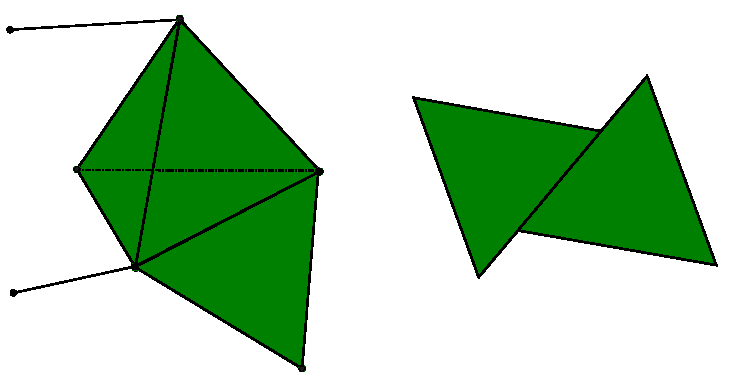
\includegraphics[width=0.4\textwidth]{compare.pdf}
 \caption{\label{fig:compare} The shape on the left is a simplicial complex; the shape on the right is not since the triangles do not entirely share an edge.}
\end{figure}
\doublespacing
A simplicial complex can be expressed abstractly by numbering its vertices, and listing the vertex labels for each simplex in the complex. For example:
\begin{itemize}
  \item A point: $\{1\}$
  \item An edge: $\{\{1,2\},\{1\},\{2\}\}$
  \item A triangle: $\{\{1,2,3\},\{\{1,2\},\{2,3\},\{1,3\},\{1\},\{2\},\{3\}\}$
\end{itemize}
\item Let $K$ be an abstract simplicial complex, and $K^{(0)}$ be its vertex set. An \textbf{orientation}  on the simplices of $K$ is a partial order ``$<$'' on on $K^{(0)}$ so that ``$<$'' restricted to each simplex $\sigma\in K$ is a total order on $\sigma$. This means that a simplicial complex is oriented if all of the vertices in each simplex can be ordered from least to greatest (the ordering can be chosen arbitrarily), but simplices that do not share a face have their own unique ordering. 
\item Let $K$ be a finite oriented abstract simplicial complex. The \textbf{group of $n$-chains on $K$}, $C_n(K;\mathbb{Z})$, is the set of functions $\varphi:K^{(n)}\setminus K^{(n-1)}\rightarrow \mathbb{Z}$. Note that $K^{(n)}\setminus K^{(n-1)}$ is just the set of $n$-simplices inside a simplicial complex. The purpose of this construction is to let us do algebra with the simplices of a simplicial complex by associating an integer with each of them.
\item Let $\sigma\in K^{(n)}\setminus K^{(n-1)}$ where $\sigma = {u_0,u_1,\ldots,u_n}$ is a simplex with vertices $u_i$. The \textbf{boundary operator} is a function, $\partial_n(\sigma):C_n(K;\mathbb{Z})\rightarrow C_{n-1}(K;\mathbb{Z})$, defined as
\[
 \partial_n(\sigma) = \sum_{j=0}^{n} (-1)^j \{u_0,\ldots,\hat{u_j},\ldots,u_n\}
\]
where $\hat{u_j}$ denotes that the $j^{th}$ vertex has been removed. The boundary operator, $\partial_n$ is important because it ends up being equal to zero when applied to chains that do not describe the boundary of an $n^{th}$ order simplex in  $K^{(n)}\setminus K^{(n-1)}$. This leads us to our next definitions.
\item A chain $\varphi\in C_n(K;\mathbb{Z})$ is
\begin{enumerate}
 \item A \textbf{cycle} if $\partial_n(\varphi) = 0$. That is $\varphi\in ker(\partial_n) := Z_n(K;\mathbb{Z})$.
 \item A \textbf{boundary} if $\varphi\in Im(\partial_{n+1}):=B_n(K;\mathbb{Z})$.
\end{enumerate}
\end{itemize}
With the proper language in place, we can now get to homology. The $n^{th}$ homology group of a simplicial complex $K$ with coefficients in $\mathbb{Z}$ is given by
\[
 H_n(K;\mathbb{Z}) = Z_n(K;\mathbb{Z})/B_n(K;\mathbb{Z}),
\]
or in other words, it is the group of cycles modulo the group of boundaries. The dimension of the homology group is a direct reflection of the number of holes that a simplicial complex has. For example, if we stretched a circle, $S^1$, into a triangle then calculating the homology would pick up the 1-cycle going around the triangle to give $H_1(S^1;\mathbb{Z}) = \mathbb{Z}$. If we did the same process to a figure-eight, then it would pick up two 1-cycles to give $H_1(\textrm{figure-eight};\mathbb{Z}) = \mathbb{Z}\oplus\mathbb{Z}$.
% 
% To go over the algorithm of how to find the homology of a simplicial complex, take the following as an example

The full algorithm to find the homology of a simplicial complex is beyond the scope of this paper, but it can be summarized. 
\begin{enumerate}
 \item Calculate the $(n+1)^{th}$ boundary operator as a matrix. This can be done by having the rows represent the $n$-simplices in the simplicial complex, and columns that have the coefficients of the $(n-1)$-simplices that come from applying the operator.
 \item Reduce the matrices to Smith-normal form using row and column operations. Smith-normal form is achieved when the only non-zero terms are on the diagonal, and the $M_{i,i}^{th}$ diagonal divides the $M_{i+1,i+1}^{th}$ term on the diagonal. Keep track of the linear combinations of simplices that are formed by each row/column operation during this process.
 \item There is a useful theorem for $\varphi\in C_{n+1}(K;\mathbb{Z})$ which says that $\partial_{n}(\partial_{n+1}(\varphi)) = 0$. Hence, the generators of the kernel of $\partial_n$ and the image of $\partial_{n+1}$ can just be read off from the Smith-normal form matrix. By taking the generators of the kernel of $\partial_n$ modulo the generators of the image of $\partial_{n+1}$, the $n^{th}$ homology group of the simplicial complex is recovered.
\end{enumerate}

The persistence part of persistent homology requires one additional concept. A \textbf{filtration} of a simplicial complex $K$ is a sequence $\emptyset = K_0\subset K_1\subset K_2\subset \ldots\subset K_{N-1}\subset K_N = K$ such that each $K_i$ is a simplicial complex. An example is the Rips filtration, $R_\varepsilon(x)$, where given a set $X$ and a distance metric $\rho: X\times X\rightarrow [0,\inf)$ and $\varepsilon > 0$
\[
 R_\varepsilon(x) = \{\{x_0,\ldots,x_n\}|\rho(x_i,x_j)<\varepsilon, 0\leq i,j \leq n\}.
\]
In other words, the Rips filtration is given by the simplicial complexes that are generated when all points inside spheres of radius $\varepsilon$ at every point are connected. Naturally, a \textbf{filtered} simplicial complex is a simplicial complex partnered with a filtration. The persistence of a certain homology on $K$ is given by the number of sub-complexes that display that homology. 

The persistence of homologies in a filtered simplicial complex can be represented visually by a ``barcode'' that keeps track of the homologies of each sub-complex. When a new homology appears, it is said to be \textit{born}, and when it disappears, it \textit{dies}.
\begin{figure}[!htbp]
 \centering
 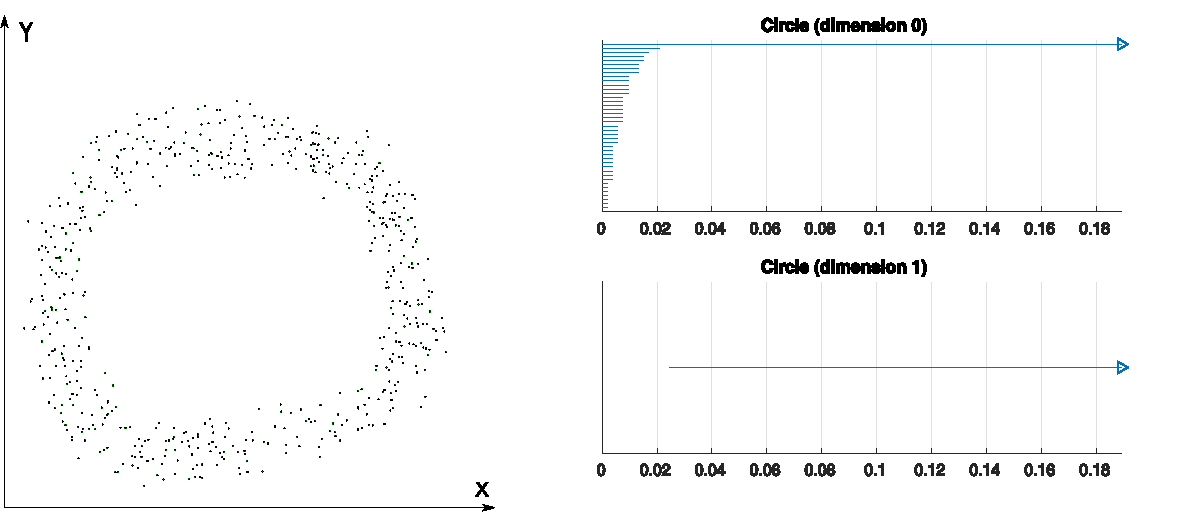
\includegraphics[width=0.8\textwidth]{circle_barcode_pc.pdf}
 \caption{\label{fig:barcode} A circular point cloud, like that on the left, generates a barcode with only one significant bar in $H_0$ and $H_1$. Barcode was generated using \textit{javaplex}\cite{Javaplex}.}
\end{figure}
\doublespacing
As can be seen in figure \ref{fig:barcode}, a point cloud with a circular distribution will start out with nothing in $H_1$, and many bars in $H_0$. This is because $H_0$ is picking up each small group of points as they are clustered together, but there are not any one-dimensional holes formed during this early clustering for $H_1$ to pick up. However, say that the Rips filtration is being used. Once $\varepsilon\approx0.025$, all of the points have been connected to enclose the hole in the middle of the circle, so a bar for $H_1$ is born, and all of the bars for $H_0$ die except one since there is now only one grouping of points. 

%%%%%%%%%%%%%%%%%%%%%%%%%%%%%%%%%%%%%%%%%%%%%%%%%%%%%%%%%%%%%%%%%%%%%%%%%%%%%%%%%%%%%%%%%%%%%%%%%%%%%%%%%%%%%%%%%%%%%%%%%%%%%

% \section{Jet Detection}\label{sec:detection}
% 
%  To accurately reconstruct the original event that formed a jet, it is necessary to find the energy, momentum, and trajectory of the secondary particles that are produced by it. Due to the variety of particles produced, there is no single detector that will work best in detecting jets. Instead, modern particle detectors employ multiple detection technologies, and properties of the particles detected are determined with the composite data collected. Since there are many different ways of building such a detector, I will use the ATLAS detector at the LHC as an example of how such a device can be used to detect jets.
% \begin{itemize}
%   
%   \item Inner detector
%   
%     The ATLAS detector has four major components: the inner detector, the electromagnetic calorimeter, the hadronic calorimeter, and the muon spectrometer. 
%   
%   The inner detector designed to track charged particles as they exit the interaction point of the detector. A 2 T magnetic field is applied to the detector, causing the trajectories of charged particles to curve via the Lorentz force by an amount proportional to their charge-to-mass ratio. As they move through the detector, these charged particles interact with three different components. The first and second are the pixel and semiconductor trackers (SCTs) respectively, which are each semiconductor detectors. Both parts use silicon as an interaction medium, and detect particles by picking up the current that is produced when charged particles passing through the silicon liberate electrons. The third part is the transition radiation tracker (TRT). It consists of an array of 4 mm diameter straw tubes filled with a xenon-based gas mixture and a high voltage wire running down the center of each tube. As charged particles ionize the gas, the liberated electrons from the gas are attracted to the center wire and form a current. 
%   
%   The inner detector is good for determining the momentum of charged particles and identifying electrons. However, many of the particles in a jet are neutral or have a low charge-to mass ratio. Additionally, the inner detector does not measure the energy of the particles passing through it. To take care of these problems, the ATLAS detector uses an electromagnetic and a hadronic calorimeter. 
%   
%   \begin{itemize}
%    \item Too much focus on inner detector?
%   \end{itemize}
% 
%   
%   \item Calorimeters
% 
%   Calorimeters measure the energy of a particle essentially by stopping it completely and seeing how much energy it deposited. They are built out of dense materials that have a high probability of interacting with a particle, and usually alternate with a detector material that can pick up the products of these interactions. When a particle interacts with the atoms of the calorimeter, it causes particles to be produced or liberated. These secondary particles can then go on to interact within the calorimeter as well. This causes a \textit{shower} of particles, and the goal is to build the calorimeter thick enough to fully contain such a shower so the entire energy of the original particle that caused it can be measured. 
%   In the ATLAS detector outside of the inner detector is the 53 cm thick ( >22 radiation lengths ) electromagnetic calorimeter, which was built primarily to measure the energy of electrons and photons. It uses lead as the absorption medium and liquid argon as its detection medium. 
%   
%   Outside of the electromagnetic calorimeter is the hadronic calorimeter, which is the most important part of the detector for seeing jets. Most of the hadrons from a jet at the center of the detector are able to pass through the detector up to this point, but this calorimeter is built to absorb these particles and their showers. It uses steel as its absorption material and scintillating tiles for detection. It is nearly 2 meters thick for a total of 9.7 interaction lengths ( the mean distance traveled for a hadron to undergo a reaction with a nucleus ). 
%   
%   \begin{itemize}
%     \item Go over types of interactions inside calorimeters?
%   \end{itemize}
%   
%   The last part of the detector is the muon system. Since muons are much more massive than electrons, they can usually pass through the detector up to this point without losing much of their energy. The system works similarly to the TRT, using a 4T toroidal superconducting magnet system to bend the muon trajectories, and larger monitored drift tubes (MDTs) (instead of straw tubes) for detection. While not directly involved in detecting jets, since the muon system is quite selective in what it detects (muons) it serves to understand event types that produce both jets and high-energy muons. 
%   
%   
%   \item How to decide what jets to keep for analysis (triggering)
%   Once particles can be detected and their various properties determined, another problem arises. In the ATLAS detector, the LHC sends bunches of $~10^8$ protons at each other 40 million times per second. Each time two bunches cross, about 20 proton-proton collisions occur. The technology to accurately measure and store the information from each event simply doesn't exist. To deal with this, the information from the detector is sent to three levels of triggers that essentially filter out all but the most interesting events. The first two triggers use field programmable gate arrays (FPGAs) to deal with the high rate of data, while the last trigger uses a cpu farm to pick out only the most interesting events. The three trigger levels bring the rate of data from hundreds of millions of events per second, down to about 200 events per second, which are then stored for analysis. 
%   
%   \begin{itemize}
%   \item Trigger level analysis?
%   \item More on how the triggers work?
%   \end{itemize}
%   
% \end{itemize}

\section{Jet Analysis}\label{sec:ja}
Jets are seen in particle accelerators as a roughly grouped set of particles with momenta aligned in a similar direction. Currently, researchers have a few different ways to determine how to cluster these particles so that they correspond with the original quark or gluon that spawned them. The most successful of these techniques has been the sequential jet clustering algorithms. These algorithms all work very similarly, with the main difference being their treatment of the weighting of the distance measure by momentum. The general algorithm goes as follows\cite{salam:2011}:
\begin{enumerate}
 \item Take a pair of particles $i$, $j$ and calculate the distance measure between them
 \[
  d_{ij} = \min(p_{ti}^{2l},p_{tj}^{2l})\Delta R_{ij}^2/R^2
 \]
 and the distance measure between particle $i$ and the beam
 \[
  d_{iB} = p_{ti}^{2l},
 \]
 where $p_{t}$ is the component of the momentum of a particle that is perpendicular to the beam (a.k.a. the transverse momentum), and $R$ is the jet-radius parameter, usually taken to be about $1$. $\Delta R_{ij}^2 = (\eta_i-\eta_j)^2 + (\phi_i-\phi_j)^2$ is the distance between the particles in azimuth-pseudorapidity space. Note that pseudorapidity is defined as $\eta = -\ln\left[\tan(\frac{\theta}{2})\right]$.
 \item Find the minimum distance measure out of all $d_{ij}$ and $d_{iB}$. If the minimum is a $d_{ij}$, merge the particles by summing their four-momenta. If the minimum is a $d_{iB}$, then particle $i$ is declared a jet and removed from further clustering.
 \item Repeat these steps until no particles are left.
\end{enumerate}

The type of clustering algorithm depends of the value of $l$:
\singlespacing
\begin{itemize}
 \item Kt algorithm: $l=1$
 \item Cambridge-Aachen(CA) algorithm: $l=0$
 \item Anti-kt algorithm: $l=-1$
\end{itemize}
\doublespacing
Each algorithm has its own advantages and disadvantages, and their use depends on how momentum should be treated for a particular analysis. In general, the anti-kt algorithm is used if circular jets are desired, while the CA algorithm is good for looking at jet substructure. 

One of the biggest problems in jet clustering arises when a massive relativistic particle is produced. In their rest frame, if these particles decay into two jets, the jets will emerge back-to-back. However, since they are highly relativistic, or boosted, the jets can emerge from the decay nearly on top of each other. We cannot throw out events with such particles because in many cases, they are exactly what we are looking for. As we look for new physics, we will be interested in the properties of heavy particles such as top quarks, and heavy particles that are theorized only to exist at high energies.

A common technique to deal with this problem is to perform an analysis on how the jets were clustered. Typically, the CA clustering algorithm is used to construct jets with a large radius. The clustering on these large-R jets is then run backwards to pick out the major subjets -- the four-momentum sum of particles grouped together by the clustering algorithm -- that were clustered last. The positions and momenta of these subjets can then be run through a substructure variable that is sensitive as to whether or not the subjets are spread out like the top quark event in figure \ref{fig:subjets}. See reference \cite{Thaler:2010} for an example.

\section{Persistent Homology for Jets}\label{sec:tdajet}
Persistent homology probably won't work to replace clustering algorithms. The sequential clustering algorithm works very quickly, with computation time increasing quadratically with the number of particles in an event. However, computing the persistent homology involves reducing a boundary matrix to Smith-normal form, where computation time increases cubically with the number of simplices. Since high energy physics analyses often deal with millions of events at once, calculating the persistent homology of all of them would be impractical, unless a more efficient algorithm is found.

However, persistent homology may be useful in improving jet clustering algorithms. Computing it for an event reveals the distance scale at which structures and substructures of the event live. Hence, the persistent homology of events may be able to be used to define a variable jet radius for clustering algorithms based on some other quantity, such as their energy or transverse momentum. Doing so could provide a viable alternative to the current jet substructure methods. This bring up the question: How well does persistent homology interpret jet structures?

One situation where this can be tested is in distinguishing top jets from regular QCD jets. Top quarks have an extremely short lifetime, so when they decay into jets, the daughters are still relatively close to the original collision vertex. 

\begin{figure}[!htbp]
 \centering
 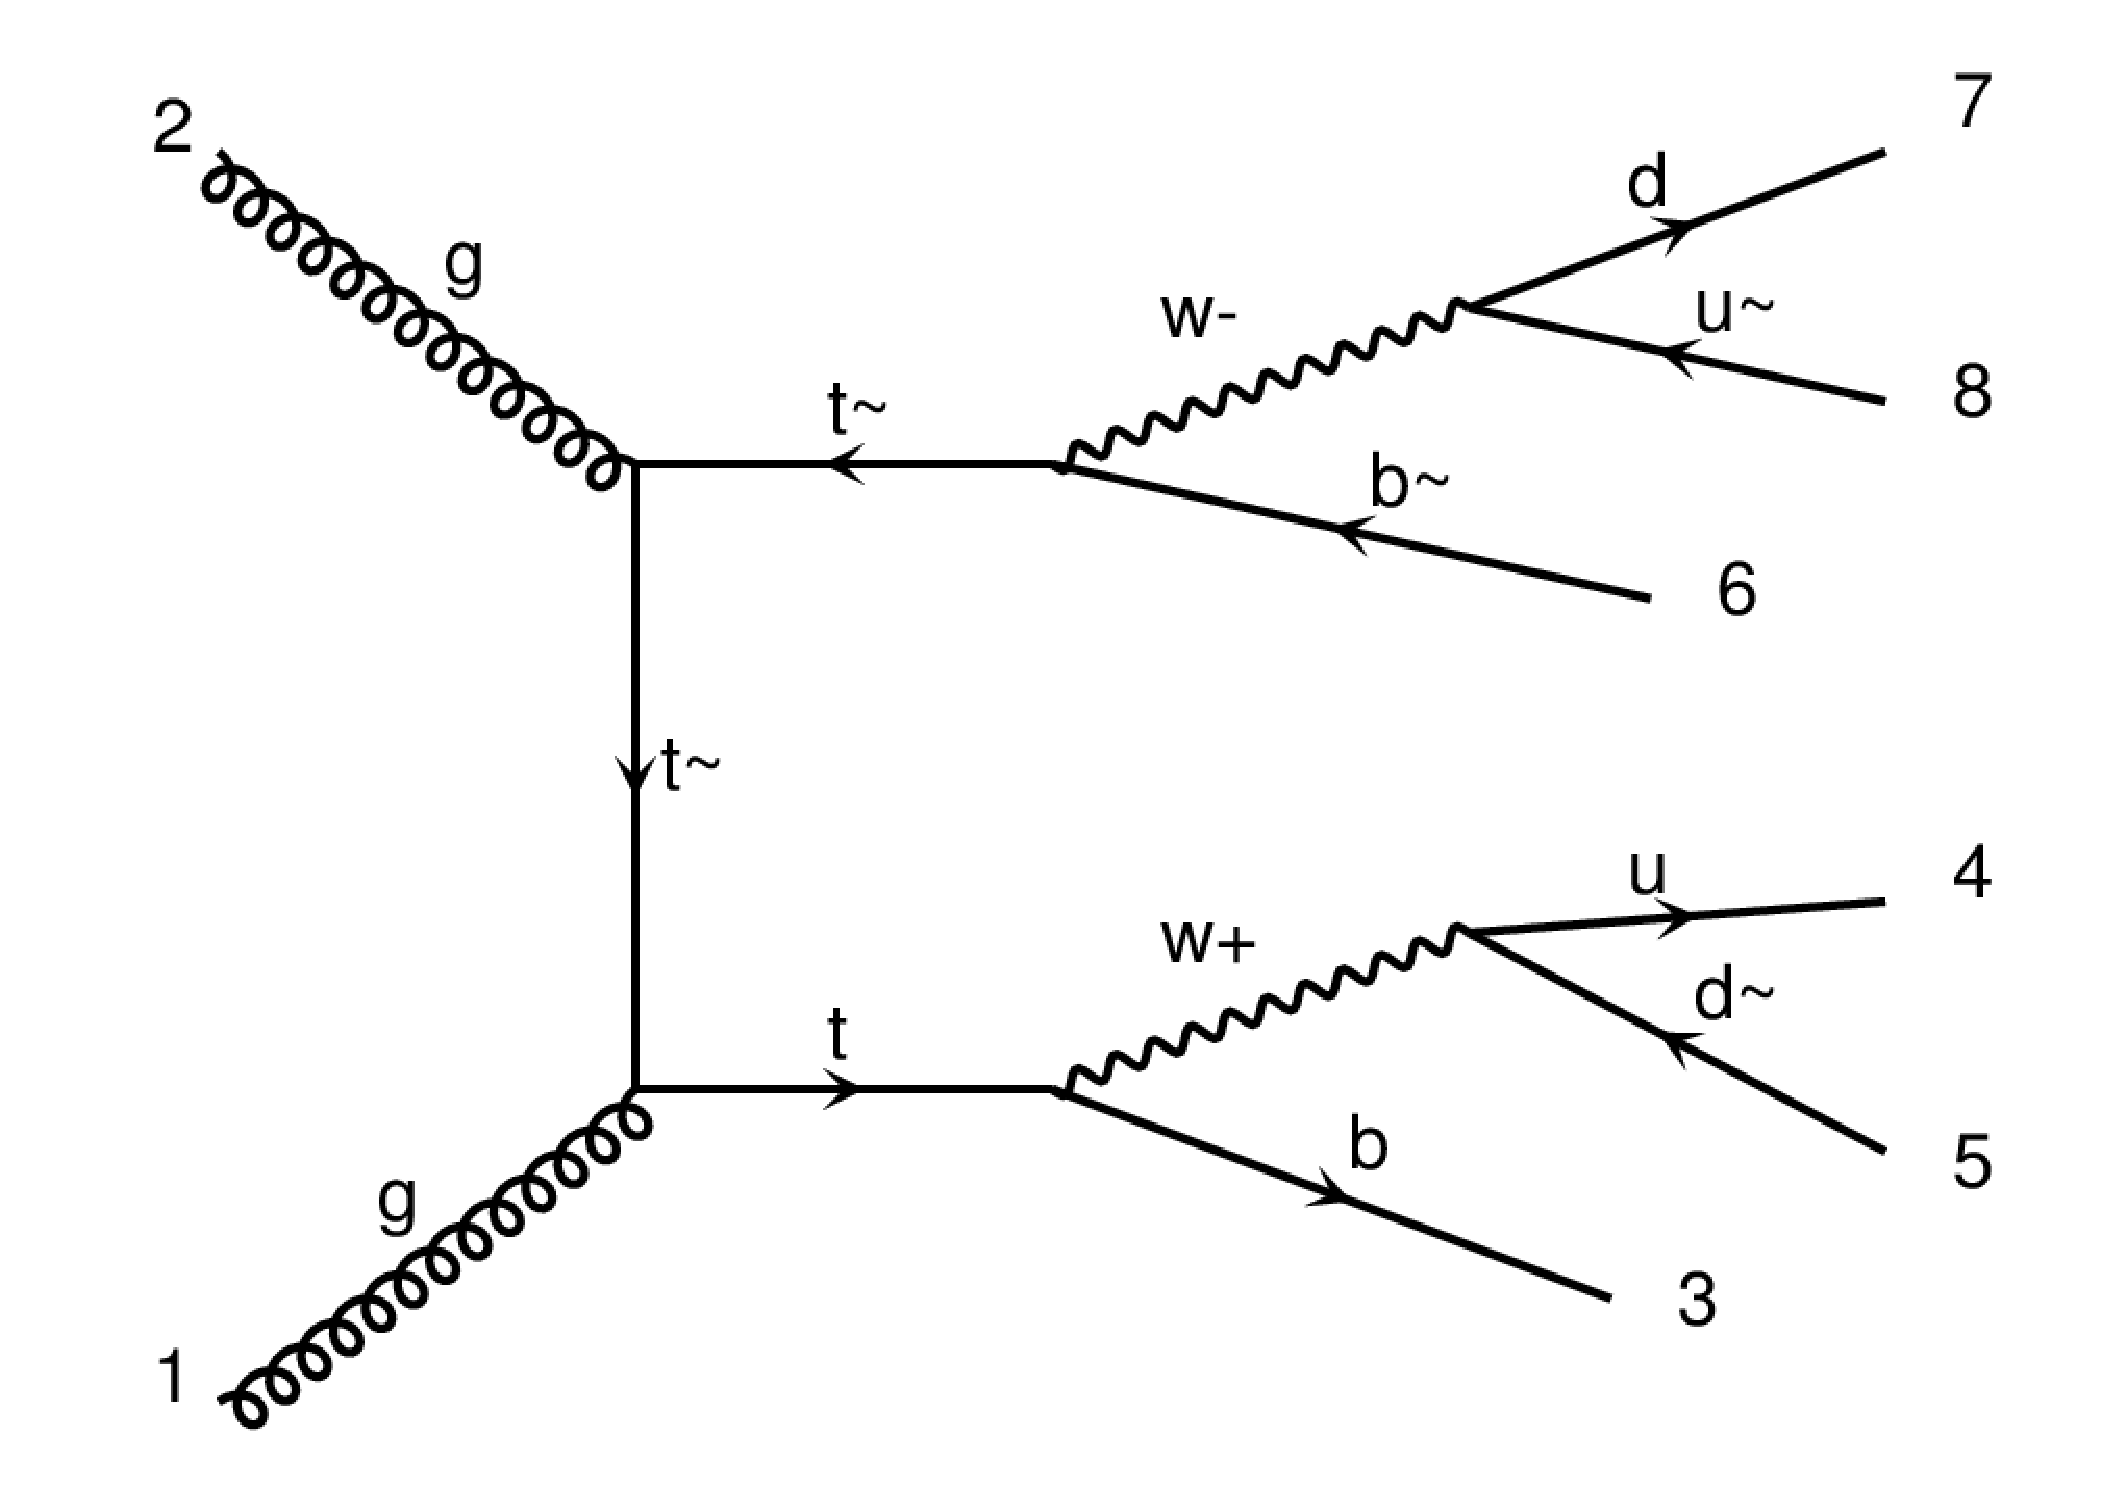
\includegraphics[width=0.6\textwidth]{ttbar.pdf}
 \caption{\label{fig:ttbar} Top quarks can decay quickly into three lighter quarks, each of which form a jet. Diagram made by Madgraph5\_aMC@NLO.}
\end{figure}

This means that each top quark is distinguished by having three separate jets that exit the event next to each other. Other QCD particles (quarks and gluons) will not decay so quickly, so their jets will not have these three distinct prongs.

\begin{figure}[!htbp]
 \centering
 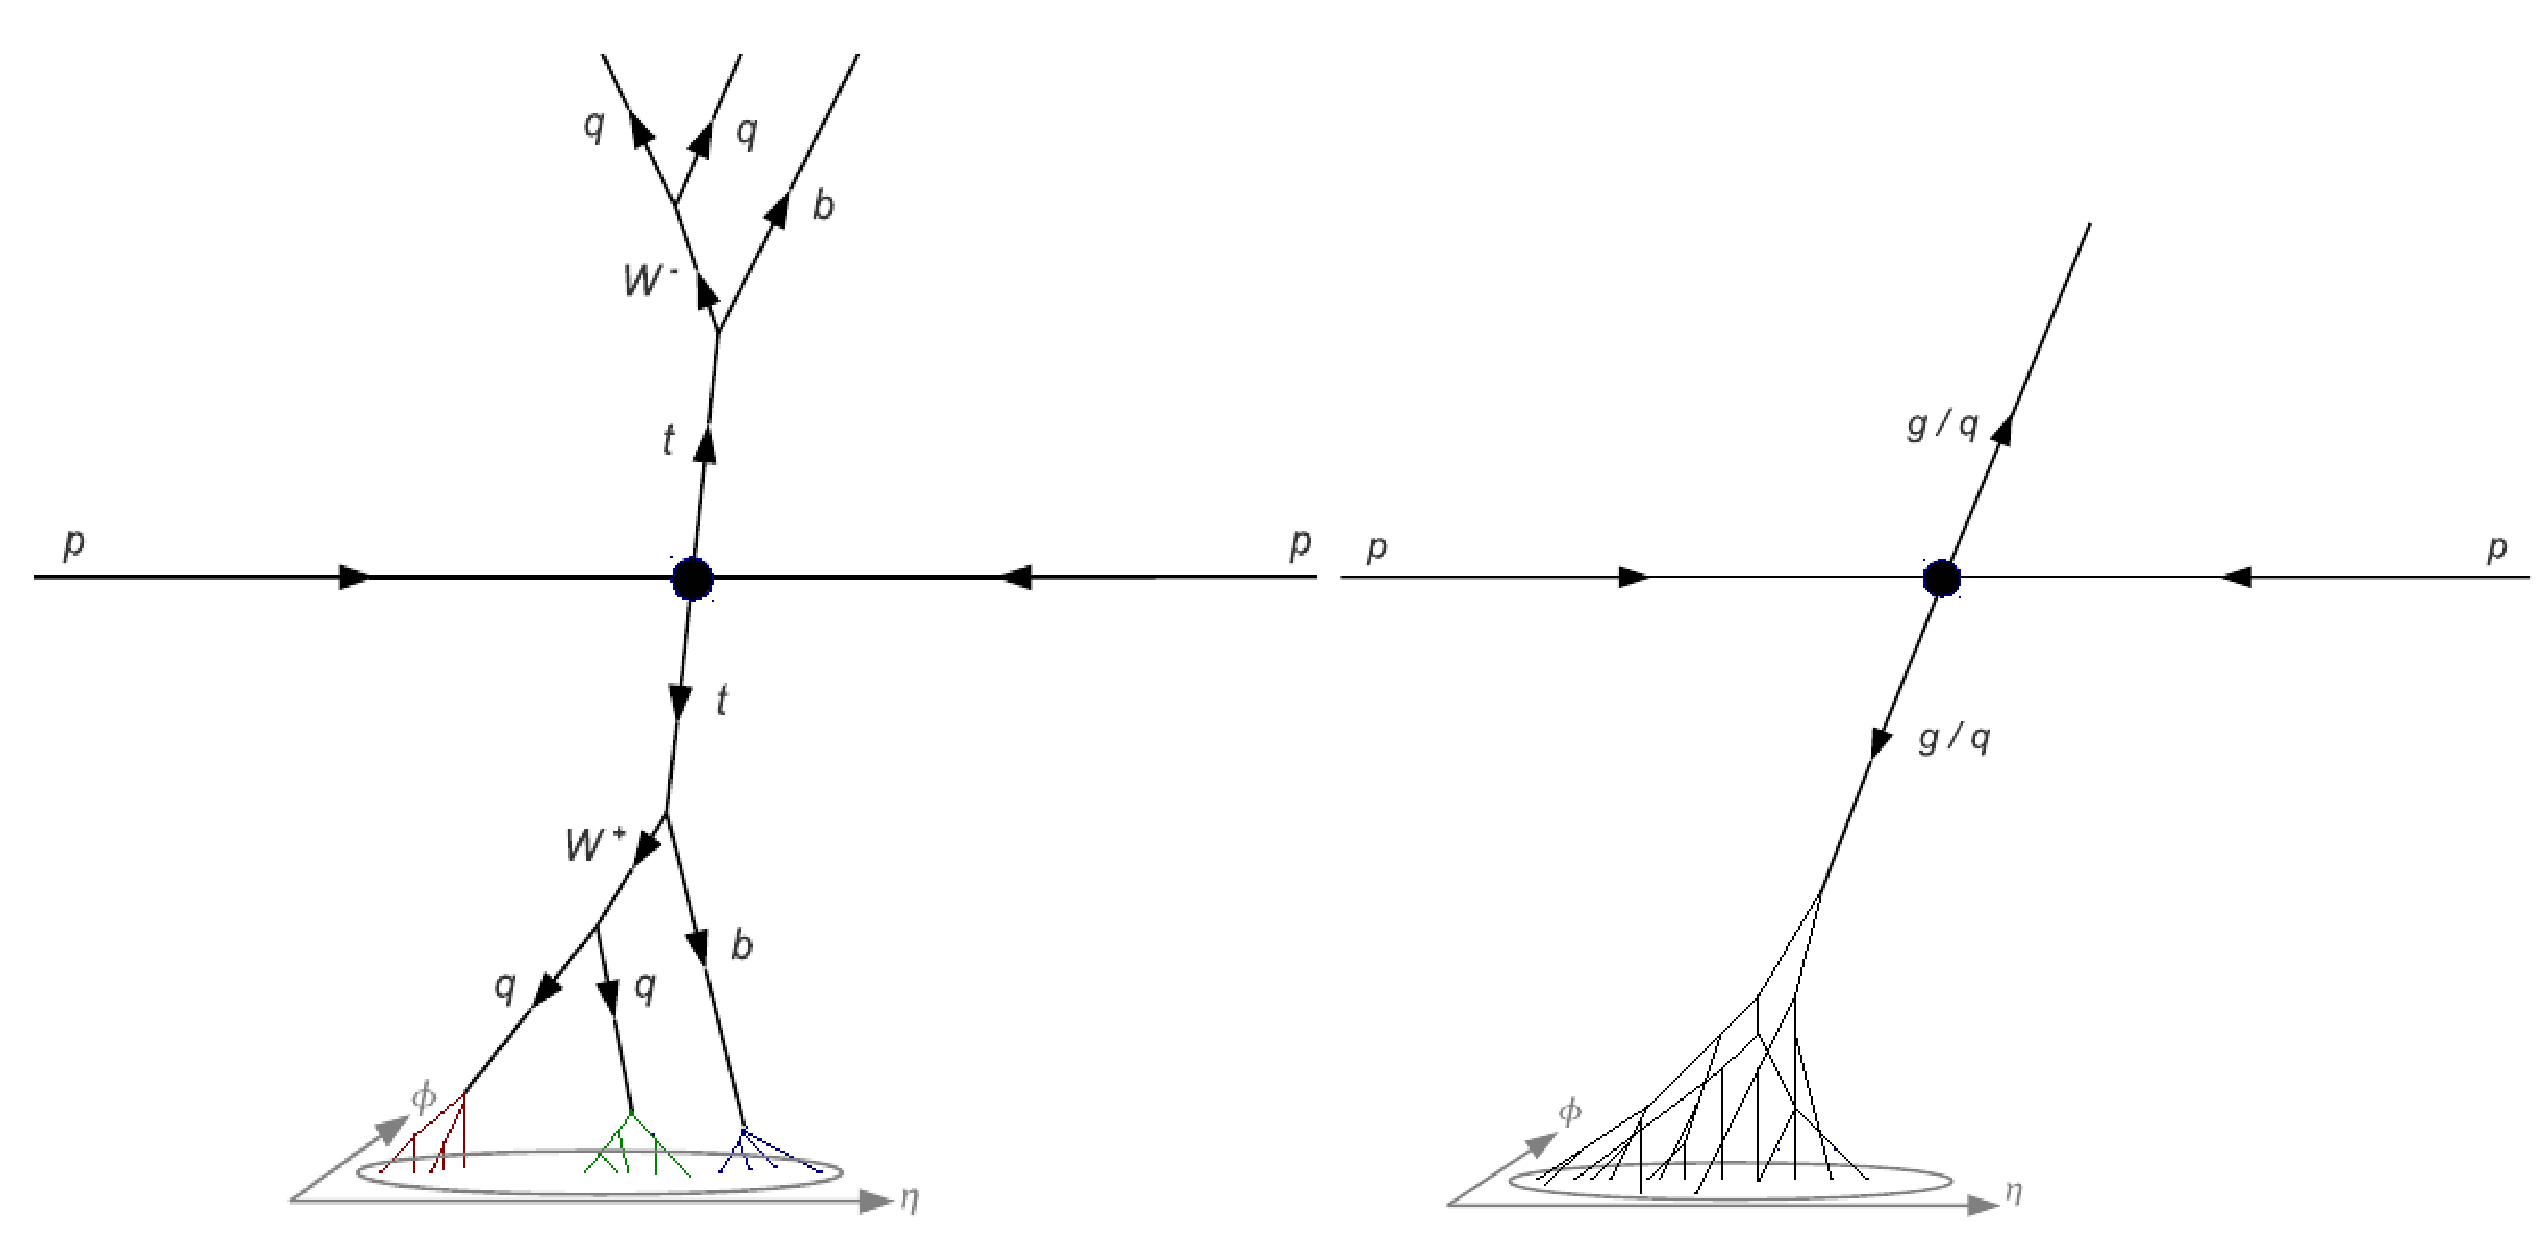
\includegraphics[width=0.8\textwidth]{jets.pdf}
 \caption{\label{fig:subjets} Top quarks decaying to jets have three prongs (left), while QCD jets with invariant mass near that of the top quark can have fewer prongs (right). Figure from reference \cite{Thaler:2010} }
\end{figure}

To look at such events, the following procedure was used to generate their point clouds and calculate the persistent homology:
\begin{enumerate}
 \item The Madgraph Monte-Carlo event generator was used to generate $t\bar{t}\rightarrow jets$ events and QCD jet events separately \cite{madgraph:2011}. Pythia \cite{Pythia:2006} was used to calculate the hadronization of these particles into jets. 
 \item Events were ``cleaned'' so that the major jet features were more prominent. (1) Only particles with no daughters were kept, since these are the particles that would be seen in the detector. (2) The $\eta-\phi$ distance between each pair of particles was arranged into a distance matrix. (3) Particles with $\eta > 4.0$ were thrown out since they would be nearly parallel with the beam. (4) Isolated particles where $\Delta\eta^2+\Delta\phi^2 > 4.0$ with their nearest neighbor were thrown out since they would not be clearly in any jet.
 \item The persistent homology was calculated on the remaining distance matrix. 
\end{enumerate}

The Rips filtration was used for calculating the persistent homology because it is sensitive to the structure of the denser areas of the point cloud. Initially, \textit{javaplex} \cite{Javaplex} was used for calculating the homology, but it was too computationally expensive to use for iteration ( For the events that were calculable, it made simplicial complexes with $>10^6$ simplices.). Instead, \textit{TDATools} \cite{TDA} was used. This software uses a Rips-collapse algorithm that generates the same diagrams as the Rips filtration, but is considerably faster. It has the disadvantage of only being able to calculate up to $H_1$, so only the two-dimensional $\eta-\phi$ space was used in building the event point clouds.

% \begin{figure}[!htbp]
%  \centering
%  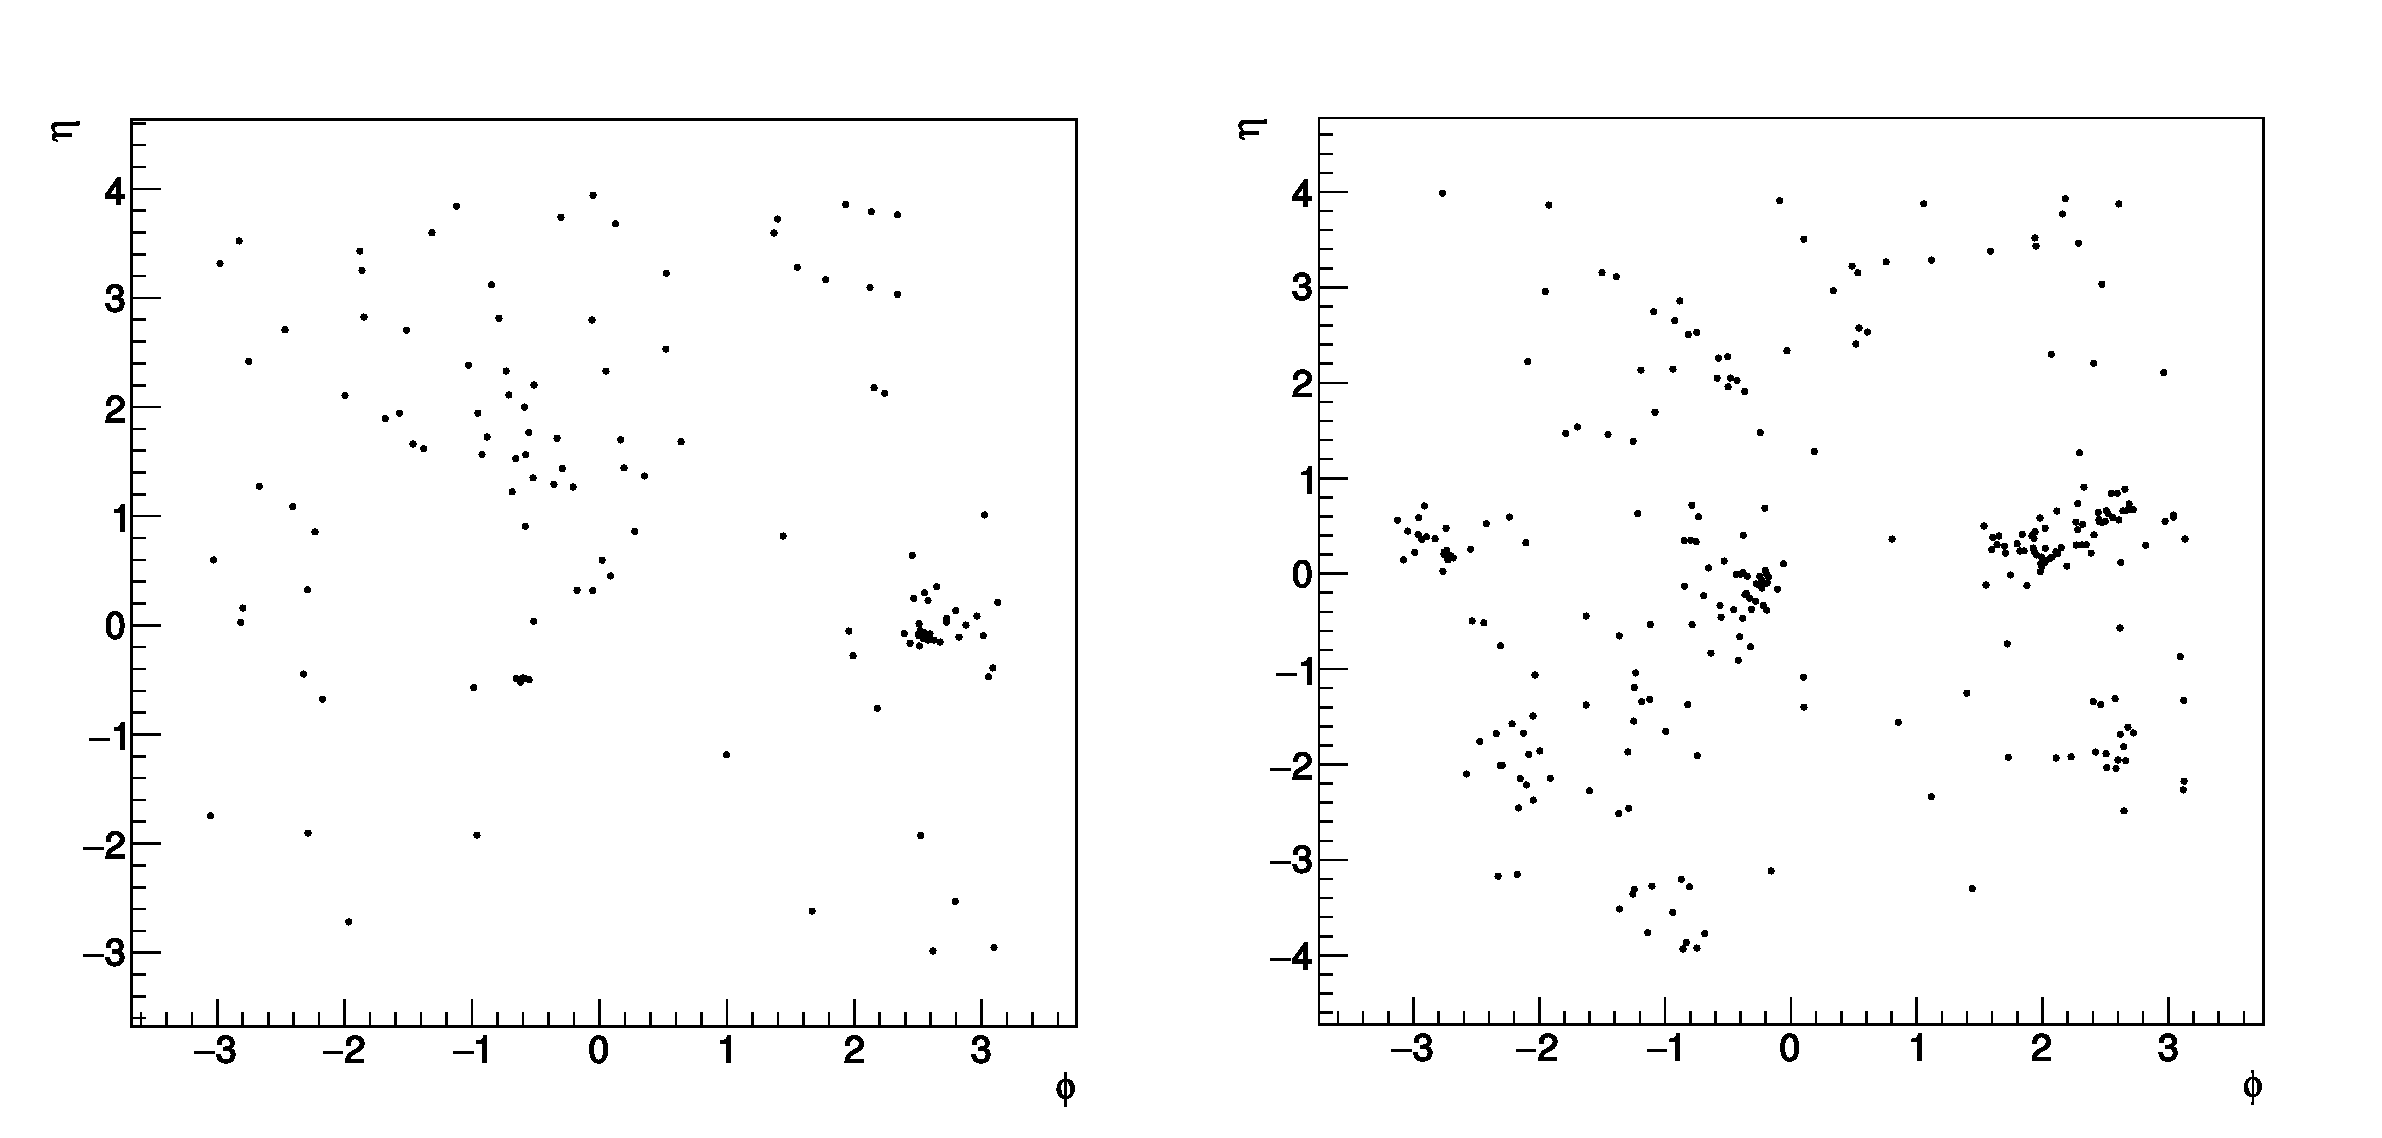
\includegraphics[width=0.8\textwidth]{point_clouds.pdf}
%  \caption{\label{fig:points} Point clouds in $\eta - \phi$ space for a QCD jet event (left) and a $t\bar{t}\rightarrow jets$ event (right). }
% \end{figure}

Typical results for events are shown in figures \ref{fig:H0} and \ref{fig:H1}. They are formatted as \textit{persistence diagrams}. Note that these carry the same information as the barcode example of section \ref{sec:ph}, only the birth of a feature is represented on the horizontal axis, while the death of a feature is represented on the vertical axis. Hence, the most significant features of the point cloud will be those farthest from the diagonal.

$H_0$ shows much more structure for the $t\bar{t}\rightarrow jets$ event, with $\approx6$ subjets showing up as expected. The QCD jet event has two main features for $H_0$, as expected for two jets leaving the collision back-to-back. Note that the point at $-1$ represents the point at infinity; this is due to $H_0$ picking up the entirety of each point cloud. $H_0$ also appears to be useful in finding the jet radius, as desired. There is a clear gap between the deaths of the initial clustering of particles, and the deaths of the jets/subjets.

\begin{figure}[!htbp]
 \centering
 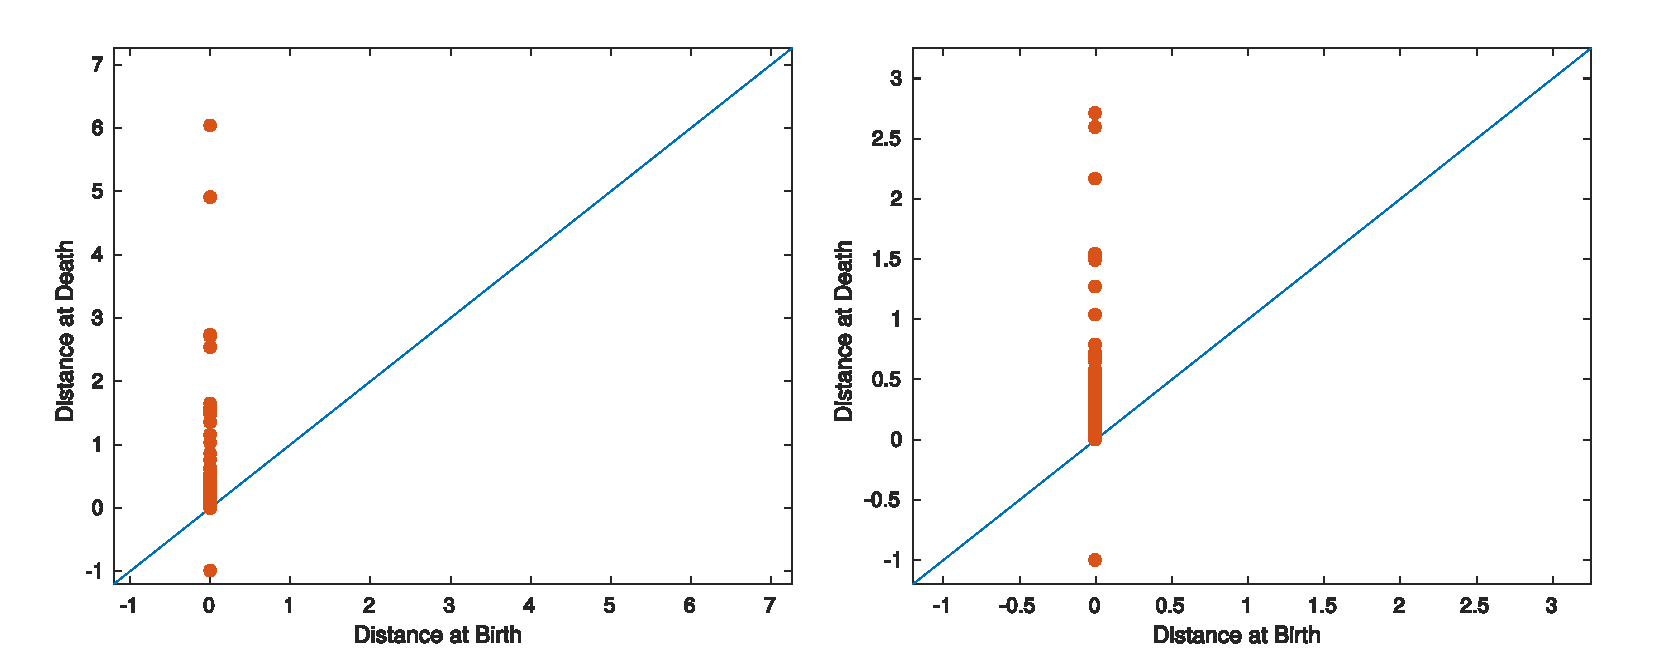
\includegraphics[width=0.8\textwidth]{H0_both.pdf}
 \caption{\label{fig:H0} Persistence diagram for $H_0$ for a QCD jet event (left) and a $t\bar{t}\rightarrow jets$ event (right). }
\end{figure}

\begin{figure}[!htbp]
 \centering
 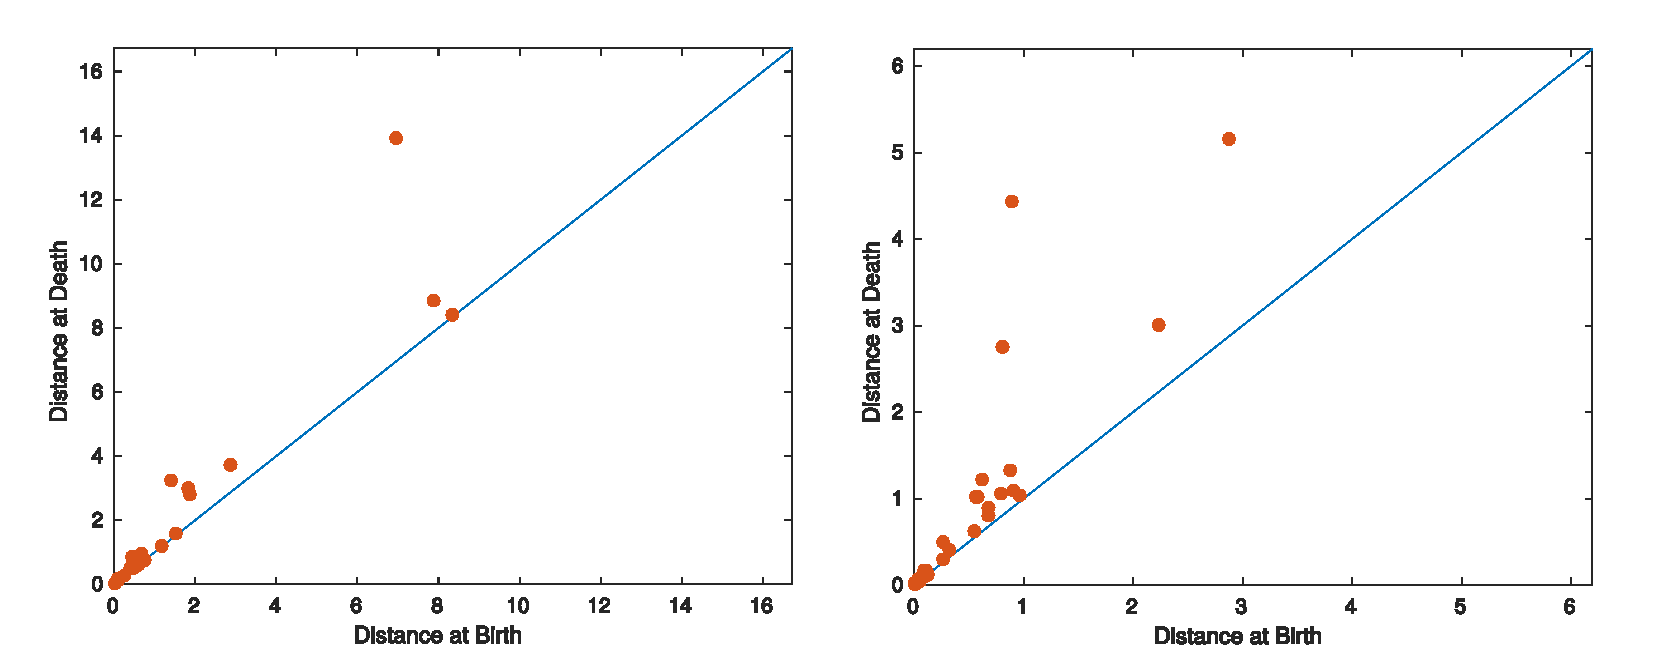
\includegraphics[width=0.8\textwidth]{H1_both.pdf}
 \caption{\label{fig:H1} Persistence diagram for $H_1$ for a QCD jet event (left) and a $t\bar{t}\rightarrow jets$ event (right). }
\end{figure}

$H_1$ ended up having more features than expected. It is possible that it is picking up the ``hole'' that is formed between the prongs of each jet as the Rips distance is increased. This would be a good way to distinguish jets with $\geq3$ prongs if that is the case. 

The next step would be to develop a metric to measure the distance between persistence diagrams for many events. This would allow us to verify that QCD jet and top jet events do indeed segregate into unique types of diagrams, and allow us to see if there is a pattern in the jet radius as a function of some other variable. 

\section{Conclusion}\label{sec:conclusion}

 It is important to understand jets because they are the dominant feature that is detected in the high-energy particle accelerators of today and tomorrow. Their simulation and analysis not only helps us understand what particles produced them, but also serve as a test of our knowledge of how QCD works. A jet is seen in a detector as a group of collimated particles. In order to recover the properties of the original quark or gluon that produced it, these particles must be clustered together as seen in section \ref{sec:ja}. 
 
%  
%  This clustering is hindered by two problems that will only become more prevalent as the LHC is upgraded and later as more powerful particle accelerators are constructed. The first problem is pileup, which occurs when particles from another event contaminate a jet. This problem can be partially dealt with by various analytical techniques, such as a check to make sure that most of the particles in a jet are sufficiently collimated, or throwing out events with jets that are close to those from another event. However, in the long run pileup may present a limit to the maximum luminosity at which particle accelerators can operate. This is a problem for searching for extremely rare events, but not so much for searching for particles at new higher energy regimes.
 
 As accelerators collide particles at ever higher energies, they will produce highly boosted standard model (SM) particles and perhaps more massive particles the will decay into highly boosted SM particles. If these particles decay into jets, then instead of being back-to-back, as in the rest frame, the highly boosted frame will cause them to enter the detector nearly on top of each other. This problem is dealt with today by clustering particles within a larger radius for highly boosted jets, and using the resolution of the detector to probe the substructure of the jet as seen in section \ref{sec:ja}.
 
 These considerations show that accelerator technology, not considering cost, will continue to be limited by our ability to analyze and detect jets. Persistent homology may be a useful tool in finding ways to improve current clustering algorithms and jet substructure tools by allowing a better understanding of jet size and structure as a function of other variables, such as energy or momentum. It was seen in section \ref{sec:tdajet} that it can be used to interpret jet structure, but methods to analyze a larger sample size need to be developed before making any conclusions.
 
\nocite{*}
\bibliographystyle{plain}
\bibliography{Project4.bib}
\end{document}          
